\section{Experiments}\label{sec:Experiments}
In this section we present the results of our experiments to demonstrate the flexibility of the SBM pipeline for top-down biodiversity modeling. The experiments are designed to answer the three research questions:
\begin{enumerate}
    \item How do different models perform compared to each other?
    \item How do models perform with different strategies of cross-validation, specifically random cross-validation vs. spatial cross-validation?
    \item How do models perform in data-limited scenarios?
\end{enumerate} 

For research question 1, we compare the performance of different models to each other. These results are presented in Section~\ref{sec:research-question-1}. For research question 2, we compare the performance of models to themselves across different cross-validation strategies, specifically 10-fold random cross-validation vs. 10-fold spatial cross-validation. These results are presented in Section~\ref{sec:research-question-2}. For research question 3, we compare the performance of models to themselvesin data-limited scenarios. These results are presented in Section~\ref{sec:research-question-3}. The models that were evaluated and compared are GLM, GAM, Random Forest, CatBoost, and FFNNs, we used the hyper-parameters that are list in Table \ref{tab:best-hyperparameters}.

\subsection{Model class comparison}\label{sec:research-question-1}
Research question 1 is concerned with how different models perform against each other. This is commonly done in the literature especially when evaluating a new model \parencite{ngor2023, cai2023, baggstrom2025}. We ran experiments comparing the performance of different models on our final 2020 UKBMS dataset described at the end of Section~\ref{subsubsec:data}. The distribution of species richness across the 2020 UKBMS dataset is shown in Figure~\ref{fig:species-richness-distribution}. We used the 15 predictor variables in Table~\ref{tab:environmental-features} at the two different spatial scales, for a total of 30 predictor variables, to predict species richness across the \(1,363\) sites.

\begin{figure}[ht]
    \centering
    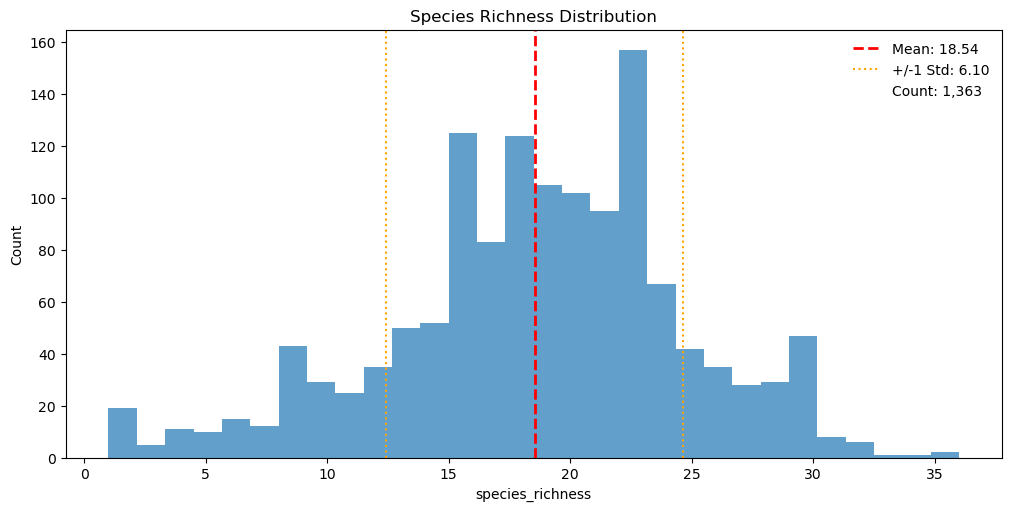
\includegraphics[width=0.8\textwidth]{
        Images/species_richness_distribution.png}
    \caption{Distribution of species richness across the \(1,363\) sites in the 2020 UKBMS dataset.}
    \label{fig:species-richness-distribution}
\end{figure}

Each model that was implemented in the SBM pipeline, GLM, GAM, random forest, CatBoost, and FFNN, was run with 10-fold random cross-validation. The same seed was used for all experiments to ensure reproducibility. The evaluation metrics used for comparison, described in Section~\ref{subsec:model_comparison} were calculated separatelt on the held-out test set for each of the 10 folds.Table~\ref{tab:random-cv-test-metric-tables} reports the mean, standard deviation, median, and interquartile range of these fold-level metric values across the 10 test folds. For SMAPE, the best model for standard deviation and median are rounded to three decimal places and the true values are included in Table~\ref{tab:smape-random-cv-test} caption.

\begin{table}[ht]
\centering
\caption{Random 10-fold cross-validation test folds performance summaries for each model class across \(R^2\), MAPE, SMAPE, and RMSE. Bold values indicate the best value within each metric table. RF = Random Forets, CAT = CatBoost, NN = Feed-Forward Neural Network.}
\label{tab:random-cv-test-metric-tables}

\begin{subtable}{0.48\textwidth}
\centering
\small
\caption{\(R^2\)}
\label{tab:r2-random-cv-test}
\begin{tabular}{lrrrr}
\toprule
\textbf{Model} & \textbf{Mean} & \textbf{Std.} & \textbf{Median} & \textbf{IQR} \\
\midrule
GLM & 0.291 & 0.069 & 0.281 & 0.118 \\
GAM & 0.312 & 0.064 & 0.324 & 0.104 \\
RF  & 0.367 & 0.082 & 0.374 & 0.103 \\
CAT & \textbf{0.374} & 0.083 & \textbf{0.397} & 0.122 \\
NN  & 0.336 & \textbf{0.061} & 0.345 & \textbf{0.068} \\
\bottomrule
\end{tabular}
\end{subtable}
\hfill\begin{subtable}{0.48\textwidth}
\centering
\small
\caption{RMSE}
\label{tab:rmse-random-cv-test}
\begin{tabular}{lrrrr}
\toprule
\textbf{Model} & \textbf{Mean} & \textbf{Std.} & \textbf{Median} & \textbf{IQR} \\
\midrule
GLM & 5.110 & 0.434 & 5.184 & 0.431 \\
GAM & 5.036 & 0.438 & 5.133 & \textbf{0.310} \\
RF  & 4.830 & 0.517 & 4.866 & 0.542 \\
CAT & \textbf{4.800} & 0.482 & \textbf{4.813} & 0.343 \\
NN  & 4.950 & \textbf{0.427} & 4.993 & 0.436 \\
\bottomrule
\end{tabular}
\end{subtable}
\vspace{1em}
\begin{subtable}{0.48\textwidth}
\centering
\small
\caption{MAPE}
\label{tab:mape-random-cv-test}
\begin{tabular}{lrrrr}
\toprule
\textbf{Model} & \textbf{Mean} & \textbf{Std.} & \textbf{Median} & \textbf{IQR} \\
\midrule
GLM & 0.446 & 0.161 & 0.463 & 0.196 \\
GAM & 0.441 & 0.161 & 0.460 & 0.197 \\
RF  & 0.436 & 0.166 & 0.446 & 0.207 \\
CAT & \textbf{0.425} & 0.160 & \textbf{0.430} & \textbf{0.177} \\
NN  & 0.427 & \textbf{0.155} & 0.440 & 0.182 \\
\bottomrule
\end{tabular}
\end{subtable}
\hfill
\begin{subtable}{0.48\textwidth}
\centering
\small
\caption{SMAPE: GLM true std = \(0.023841\), RF true median = \(0.226459\), CAT true std = \(0.024274\) and true median = \(0.22617\)}
\label{tab:smape-random-cv-test}
\begin{tabular}{lrrrr}
\toprule
\textbf{Model} & \textbf{Mean} & \textbf{Std.} & \textbf{Median} & \textbf{IQR} \\
\midrule
GLM & 0.239 & \textbf{0.024} & 0.240 & 0.023 \\
GAM & 0.235 & 0.027 & 0.232 & 0.027 \\
RF  & \textbf{0.225} & 0.027 & \textbf{0.226} & 0.026 \\
CAT & 0.227 & 0.024 & 0.226 & \textbf{0.021} \\
NN  & 0.234 & 0.026 & 0.231 & 0.027 \\
\bottomrule
\end{tabular}
\end{subtable}
\end{table}

From the results in Table~\ref{tab:random-cv-test-metric-tables} not one model class is the best across all metrics. CatBoost performs the best for mean \(R^2\), MAPE, and RMSE while Random Forest performs the best for mean SMAPE. Additionally, CatBoost has the best median across all metrics. When looking at measures of dispersion, the best model for standard deviation is the FFNN under \(R^2\), MAPE, and RMSE while the best model for SMAPE standard deviation is the GLM. CatBoost performs the best in the  interquartile range for SMAPE and MAPE, while the FFNN performs the best for \(R^2\) interquartile range, and the GAM performs the best for RMSE when looking at interquartile range. 

Looking at a box-plot of the \(R^2\) values in Figure~\ref{fig:random-cv-r2} we can see that CatBoost and random forest have similar median \(R^2\) values, which are larger than the other models. The FFNN has a noticeably smaller interquartile range compared to the other models. The GLM and GAM have lower median \(R^2\) values compared to the other models.

\begin{figure}[ht]
    \centering
    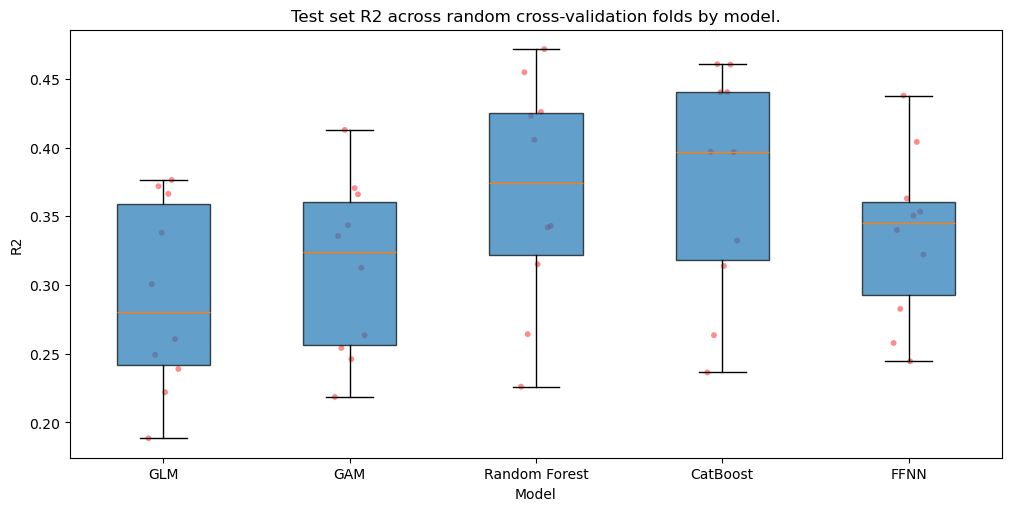
\includegraphics[width=0.8\textwidth]{Images/research_question_1/r2_randomcv_model_comparison.png}
    \caption{\(R^2\) across random cross-validation folds.}
    \label{fig:random-cv-r2}
\end{figure}

In Figure~\ref{fig:random-cv-rmse} we can see the RMSE of the models. CatBoost and random forest once again have similar median RMSE values, which are lower than the other models, but the interquartile range of the random forest is the largest and random forest has the largest range of RMSE values across the models. The GLM and GAM models have the smallest ranges of RMSE values across the models, but they also have higher median RMSE values compared to the other models. The FFNN has a slightly lower median RMSE value to the GLM and GAM, but it has a larger interquartile range and range of RMSE values across the folds compared to the GLM and GAM.

\begin{figure}[ht]
    \centering
    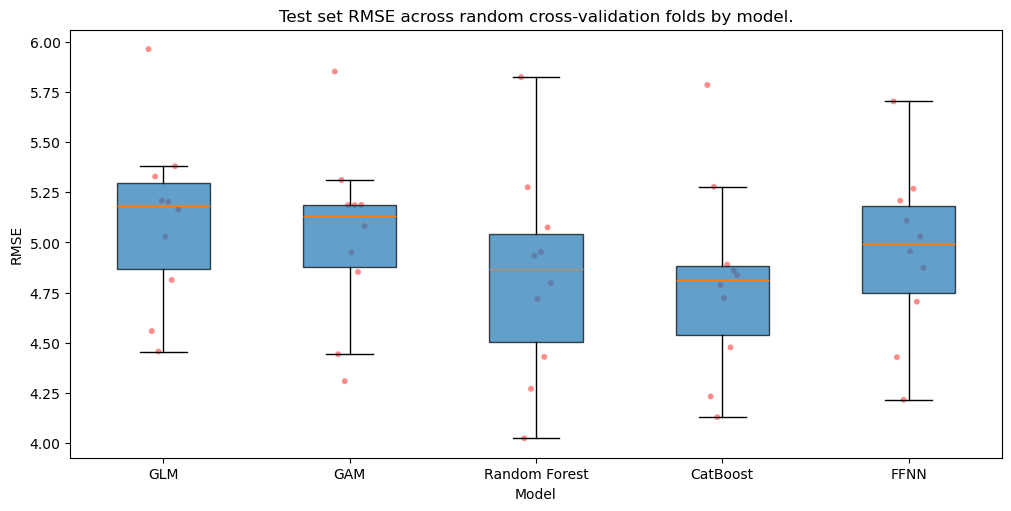
\includegraphics[width=0.8\textwidth]{Images/research_question_1/rmse_randomcv_model_comparison.png}
    \caption{RMSE across random cross-validation folds.}
    \label{fig:random-cv-rmse}
\end{figure}

In Figure~\ref{fig:random-cv-mape} we can see the MAPE of the models. All models perform very similarly in this figure in terms of mean, median and interquartile range. CatBoost barely has the lowest mean and median MAPE values. Based on the MAPE box-plot, there is no clear best model across the folds.
\begin{figure}[ht]
    \centering
    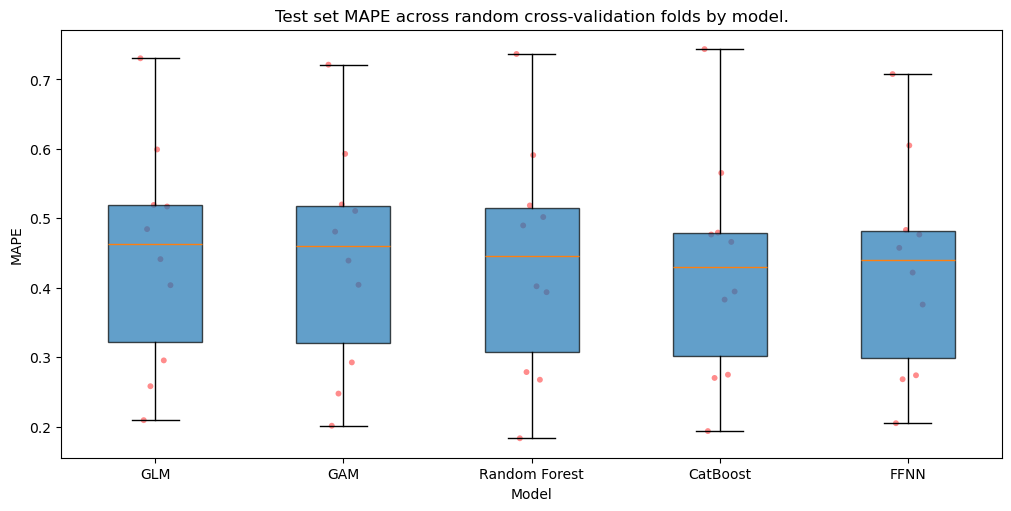
\includegraphics[width=0.8\textwidth]{Images/research_question_1/mape_randomcv_model_comparison.png}
    \caption{MAPE across random cross-validation folds.}
    \label{fig:random-cv-mape}
\end{figure}

We also look at the MAPE, SMAPE, and RMSE values across the random cross-validation folds in Figures~\ref{fig:random-cv-mape}, \ref{fig:random-cv-smape}, and \ref{fig:random-cv-rmse}. The MAPE box-plots across all models look very similar; whereas, SMAPE and RSME show a decrease in values for Random Forest and CatBoost compared to the other models. Furthermore, every models' box-plot overlap across all metrics. This would suggest that there is no single model that performs the best consistently. This is in line with much of the literature that shows that there is no single best model for all problems \parencite{mondal2021, cai2023, baggstrom2025}

In Figure~\ref{fig:random-cv-smape} we see that random forest is barely better than CatBoost in terms of median SMAPE values, but the interquartile range of CatBoost is slightly smaller than the interquartile range of random forest. The median of the FFNN is SMAPE is between the medians of the GLM and GAM and the median of the random forest and CatBoost. The GLM and GAM have similar median SMAPE values, but the interquartile range of the GAM is larger than the interquartile range of the GLM.

\begin{figure}[ht]
    \centering
    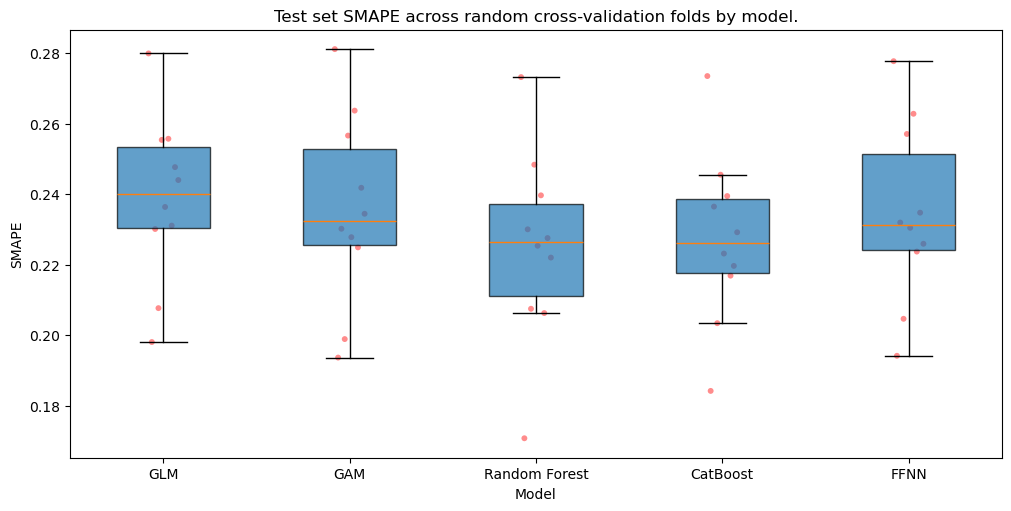
\includegraphics[width=0.8\textwidth]{Images/research_question_1/smape_randomcv_model_comparison.png}
    \caption{SMAPE across random cross-validation folds.}
    \label{fig:random-cv-smape}
\end{figure}

In addition to comparing numerical metrics across models, we can also examine the distribution of predicted species richness in the test sets relative to the distribution of observed species richness. This is shown in Figure~\ref{fig:model-species-richness-distributions}. Here we can see that all models except for CatBoost demonstrate a peak around the mean which is common among Gaussian distributions. CatBoost, however, has a slightly less dominant peak which is also not present in the true distribution. All the models demostrate a challenge in capturing the tail of the distribution. We also observe similar structures in the GLM and GAM predicted species richness distributions, which is expected as they are both statistical models. The machine learning methods, however, demonstrate fewer similarities in their predicted species richness distributions comparatively. 

Another visual check is carried out in Figure~\ref{fig:model-calibration-plots}. Here we can see the observed species richness vs. predicted species richness scatter plots for the five models. All models demonstrate a positive trend, but the strength of the trend varies across models. CatBoost and random forest demonstrate a stronger positive trend compared to the other models, which is in line with their higher \(R^2\) values. The GLM and GAM demonstrate a weaker positive trend compared to the other models, which is in line with their lower \(R^2\) values. The FFNN demonstrates a positive trend that is between the GLM and GAM and the random forest and CatBoost, which is in line with its \(R^2\) value that is between the GLM and GAM and the random forest and CatBoost in Table~\ref{tab:random-cv-test-metric-tables}. Furthermore, we can see all models have a hard time predicting high species richness values and low species richness values. The models are best at predicting species richness values around the mean, which is in line with the predicted species richness distributions in Figure~\ref{fig:model-species-richness-distributions} where all models have a hard time capturing the tails of the distribution.

\begin{figure}[H]
    \centering
    \begin{subfigure}{0.48\textwidth}
        \centering
        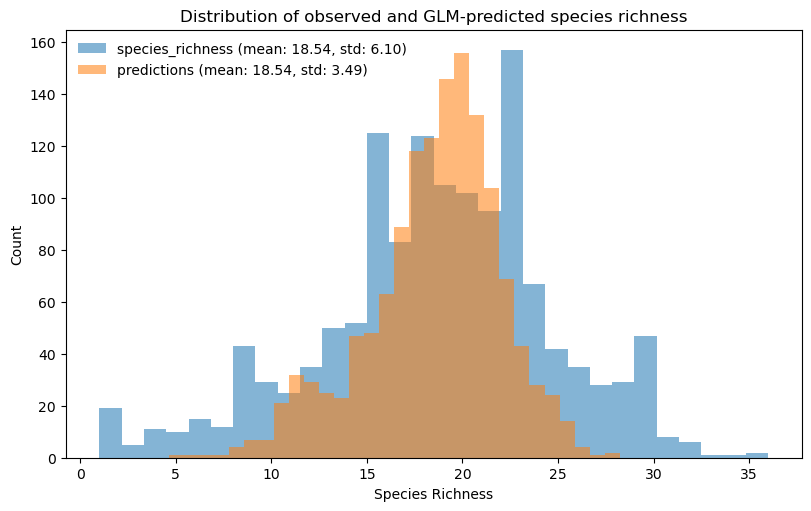
\includegraphics[width=\textwidth]{Images/research_question_1/glm_dist.png}
        \caption{GLM}
        \label{fig:glm-dist}
    \end{subfigure}
    \hfill
    \begin{subfigure}{0.48\textwidth}
        \centering
        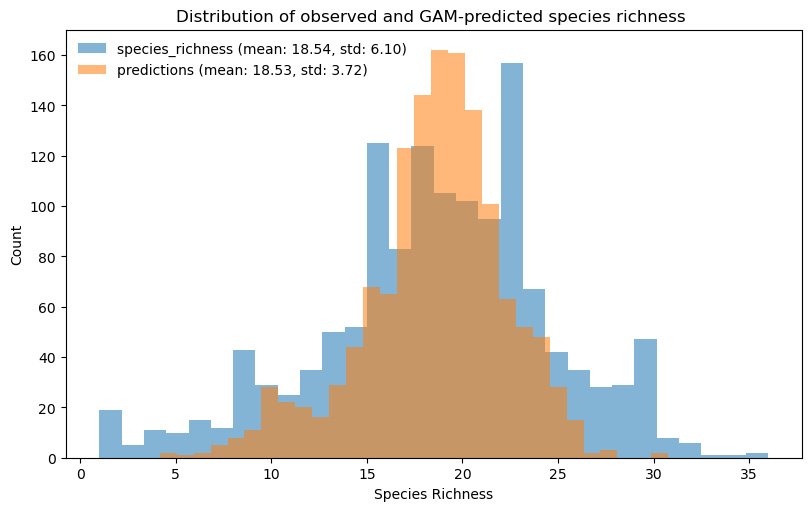
\includegraphics[width=\textwidth]{Images/research_question_1/gam_dist.png}
        \caption{GAM}
        \label{fig:gam-dist}
    \end{subfigure}

    \vspace{1em}

    \begin{subfigure}{0.48\textwidth}
        \centering
        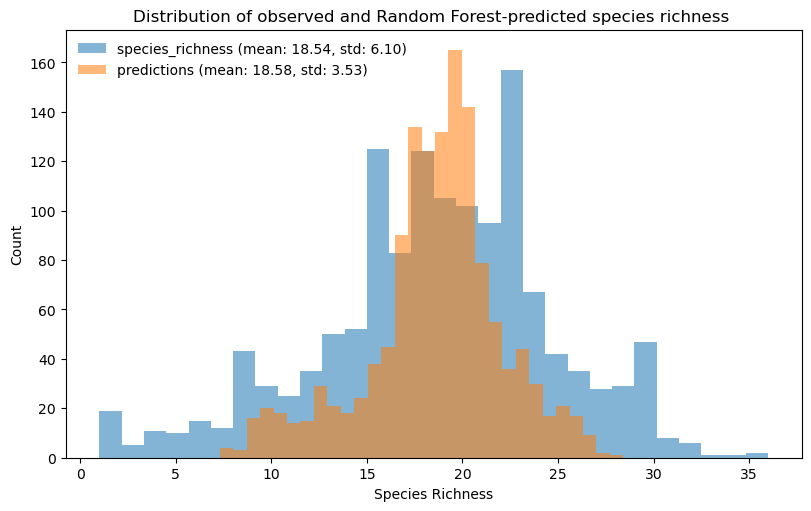
\includegraphics[width=\textwidth]{Images/research_question_1/randomforest_dist.png}
        \caption{Random Forest}
        \label{fig:randomforest-dist}
    \end{subfigure}
    \hfill
    \begin{subfigure}{0.48\textwidth}
        \centering
        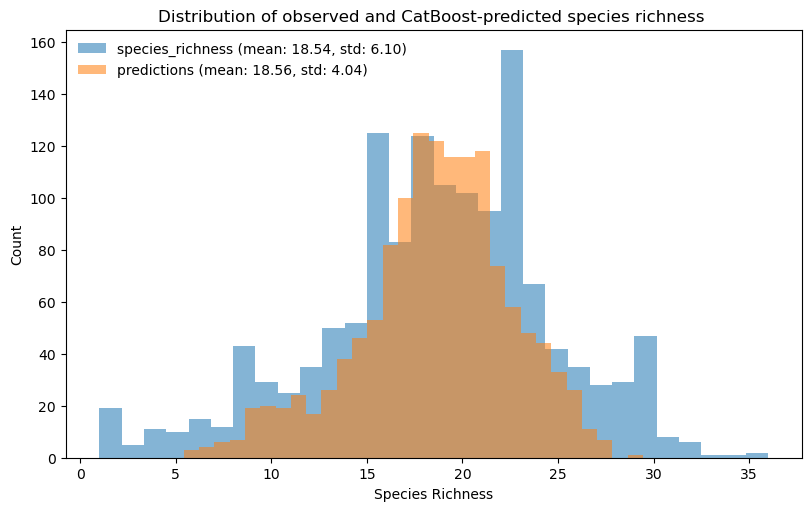
\includegraphics[width=\textwidth]{Images/research_question_1/catboost_dist.png}
        \caption{CatBoost}
        \label{fig:catboost-dist}
    \end{subfigure}

    \vspace{1em}

    \begin{subfigure}{0.6\textwidth}
        \centering
        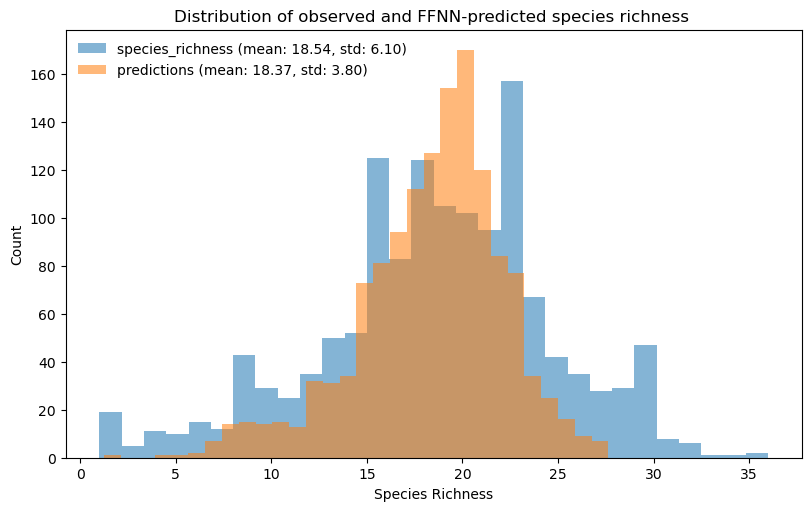
\includegraphics[width=\textwidth]{Images/research_question_1/ffnn_dist.png}
        \caption{FFNN}
        \label{fig:ffnn-dist}
    \end{subfigure}
    \caption{Observed and predicted species richness distributions for the five models, arranged in the order GLM, GAM, Random Forest, CatBoost, and FFNN.}
    \label{fig:model-species-richness-distributions}
\end{figure}

\begin{figure}[H]
    \centering
    \begin{subfigure}{0.42\textwidth}
        \centering
        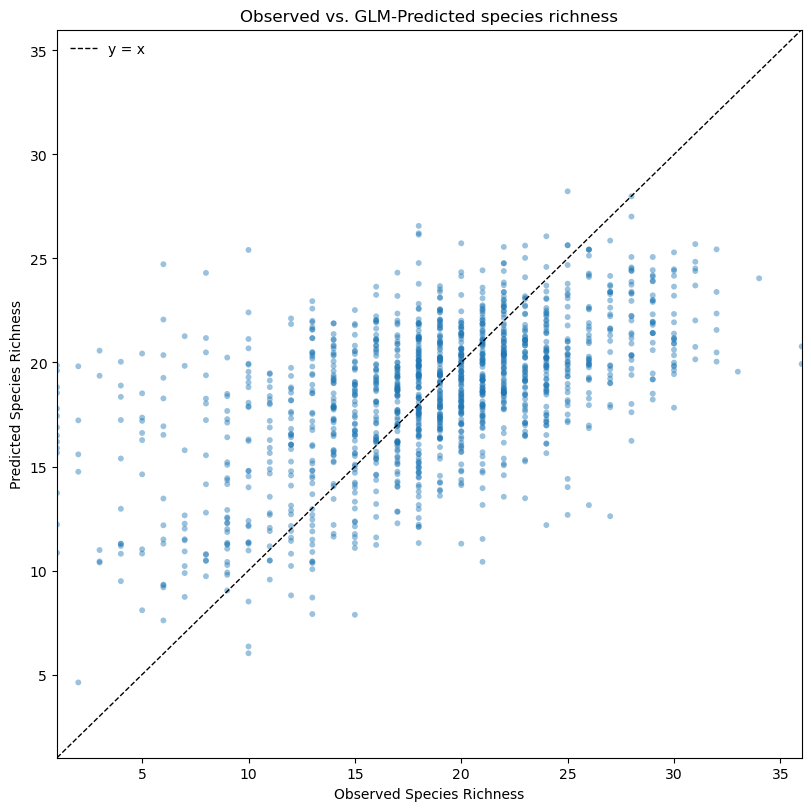
\includegraphics[width=\textwidth]{Images/research_question_1/GLM_calibration.png}
        \caption{GLM}
        \label{fig:glm-calibration}
    \end{subfigure}
    \hfill
    \begin{subfigure}{0.42\textwidth}
        \centering
        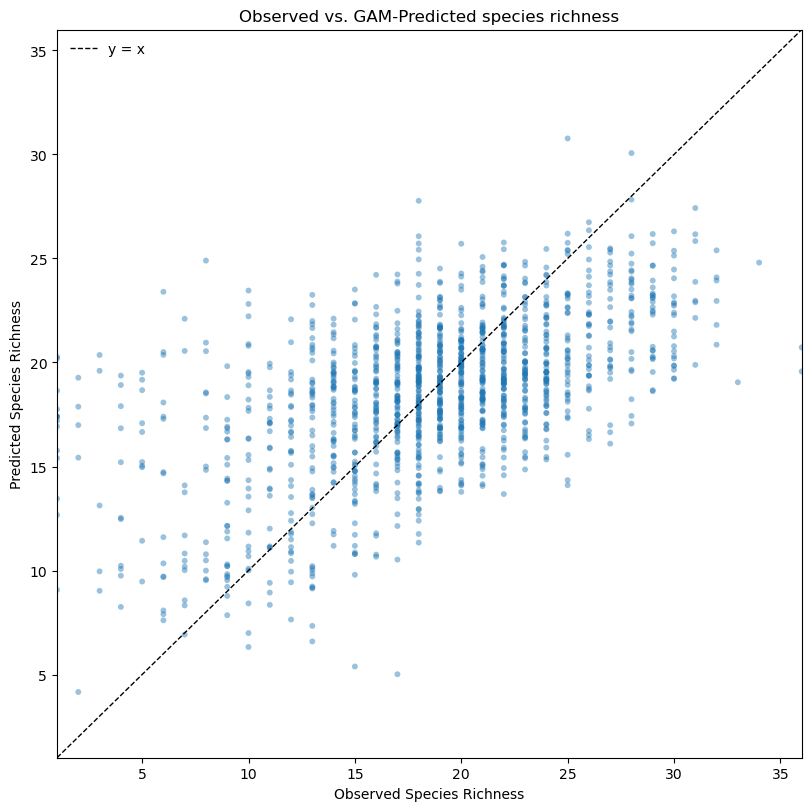
\includegraphics[width=\textwidth]{Images/research_question_1/GAM_calibration.png}
        \caption{GAM}
        \label{fig:gam-calibration}
    \end{subfigure}

    \vspace{0.5em}

    \begin{subfigure}{0.42\textwidth}
        \centering
        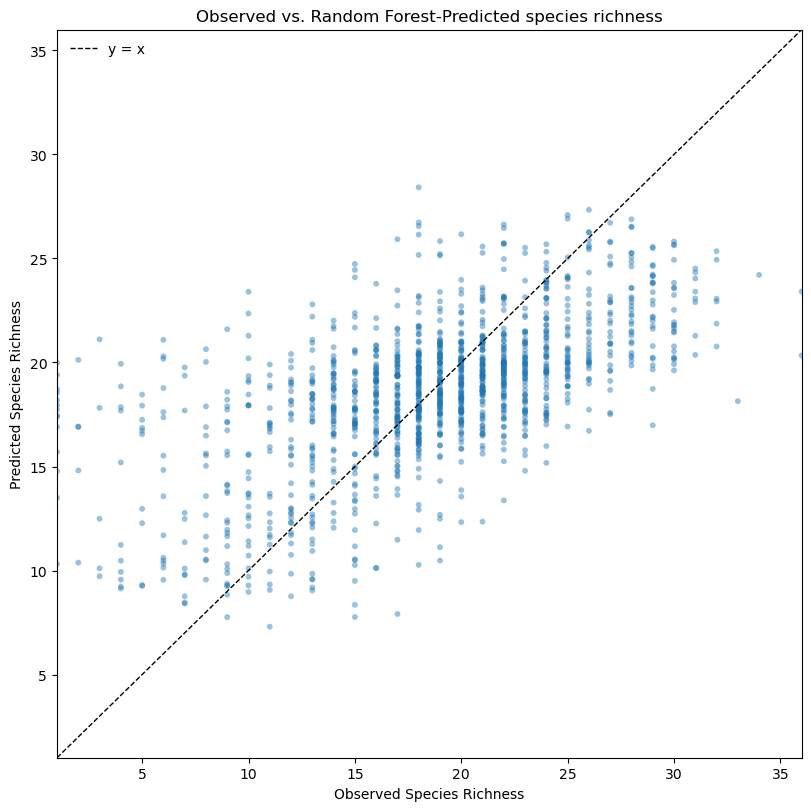
\includegraphics[width=\textwidth]{Images/research_question_1/rf_calibration.png}
        \caption{Random Forest}
        \label{fig:randomforest-calibration}
    \end{subfigure}
    \hfill
    \begin{subfigure}{0.42\textwidth}
        \centering
        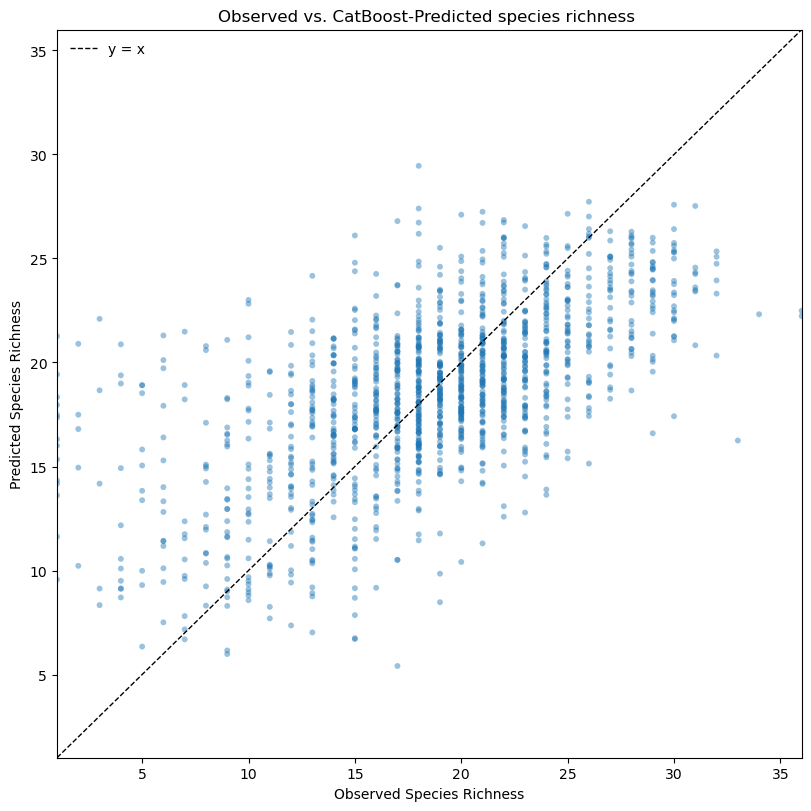
\includegraphics[width=\textwidth]{Images/research_question_1/catboost_calibration.png}
        \caption{CatBoost}
        \label{fig:catboost-calibration}
    \end{subfigure}

    \vspace{0.5em}

    \begin{subfigure}{0.42\textwidth}
        \centering
        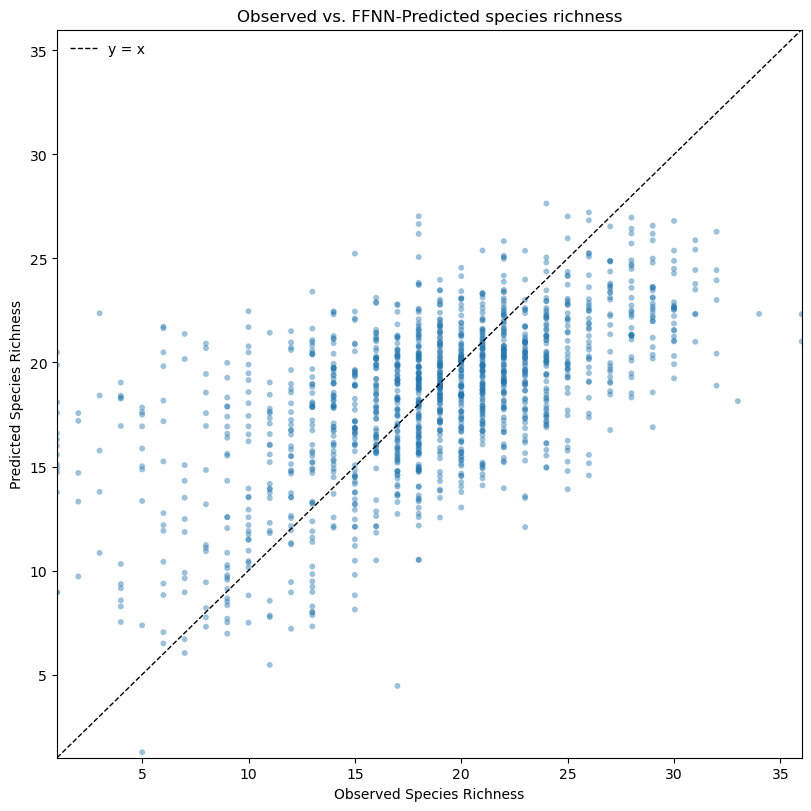
\includegraphics[width=\textwidth]{Images/research_question_1/FFNN_calibration.png}
        \caption{FFNN}
        \label{fig:ffnn-calibration}
    \end{subfigure}
    \caption{Observed and predicted species richness scatter plots for the five models, arranged in the order GLM, GAM, Random Forest, CatBoost, and FFNN.}
    \label{fig:model-calibration-plots}
\end{figure}




\subsection{Cross-validation strategy}\label{sec:research-question-2}

In this section we look at research question 2, which is concerned with how models perform across different cross-validation strategies, specifically 10-fold random cross-validation vs. 10-foldspatial cross-validation. The difference between spatial and random cross-validation for the 2020 UKBMS dataset is illustrated in Figure~\ref{fig:comparison-of-ukbms-data-distribution-across-cv-strategies} where every color corresponds to a different fold. The spatial clustering of the data is evident in Figure~\ref{fig:spatial-cv-distribution} and the random distribution of data points in the folds in Figure~\ref{fig:random-cv-distribution} are also evident. In this section we conduct comparisons of cross-validation strategies for two models, GLM and CatBoost, as one is a statistical model and the other is a machine learning model. We compare each model to itself on their performance across the two different 10-fold cross-validation strategies. Evaluations of the other models are presented in Appendix \ref{appendix:appendix_b}. An important point to note  is that 10-fold spatial cross-validation divided the dataset into unequal sizes as the sampling sites are not evenly distributed across the spatial region of interest. This can affect the calculation of the metrics across the folds if fold size is not properly accounted for. To make the comparison more robust, we will include a non-weighted, weighted, and pooled calculations for the mean and standard deviation of the metrics across the folds. The unweighted summaries treat each fold equally, while the weighted summaries weight each fold by the number of observations in its test set. The pooled calculation combines the held-out predictions from all test folds and calculates each metric once across the full set of cross-validated predictions, so that every observation is compared with its corresponding prediction.

\begin{figure}[H]
\centering

\begin{subfigure}{0.48\textwidth}
    \centering
    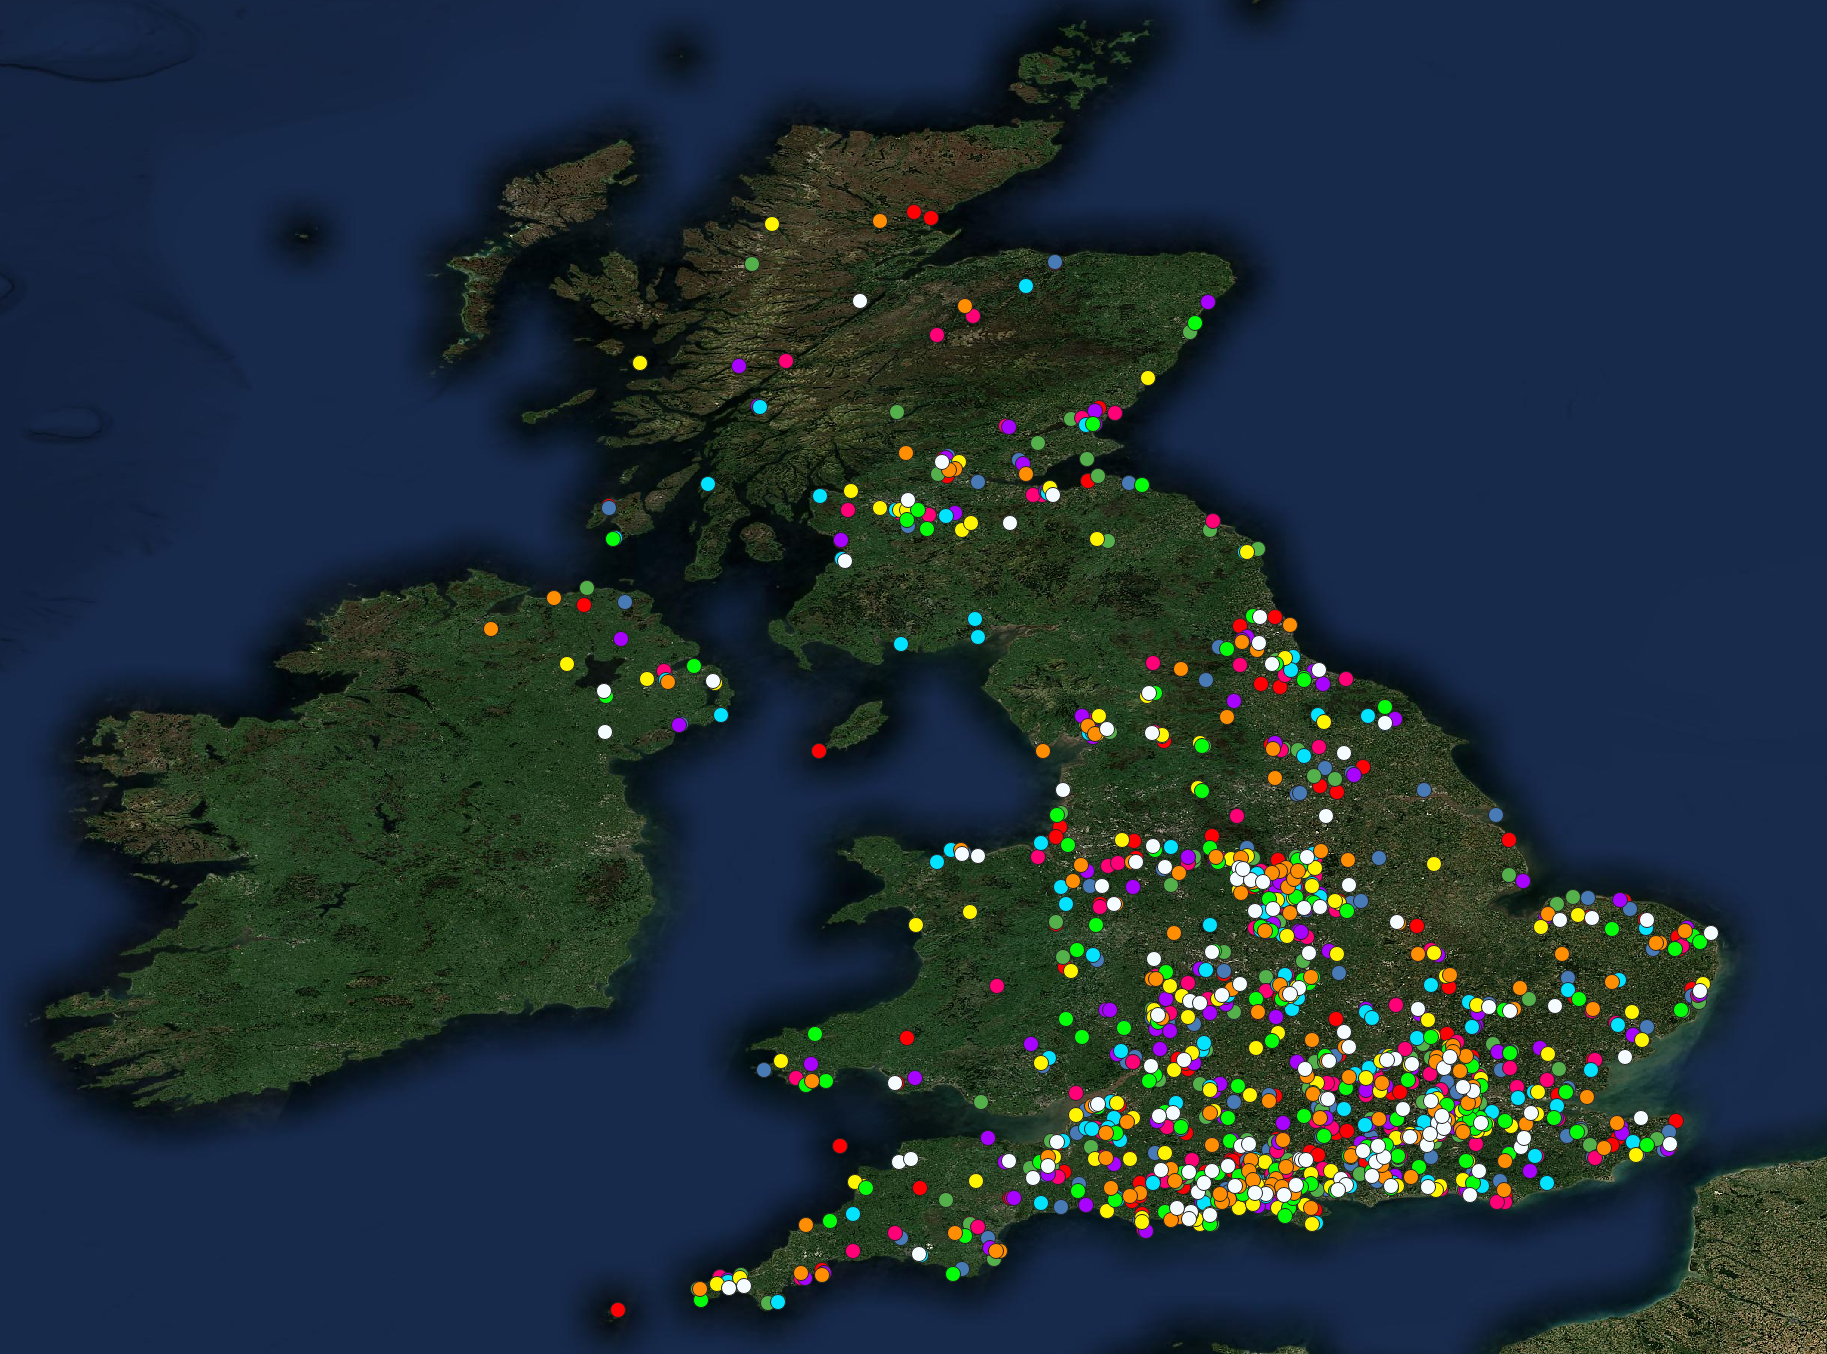
\includegraphics[width=\textwidth]{Images/Random_CV_visual.png}
    \caption{2020 UKBMS dataset - Random cross-validation folds.}
    \label{fig:random-cv-distribution}
\end{subfigure}
\hfill
\begin{subfigure}{0.48\textwidth}
    \centering
    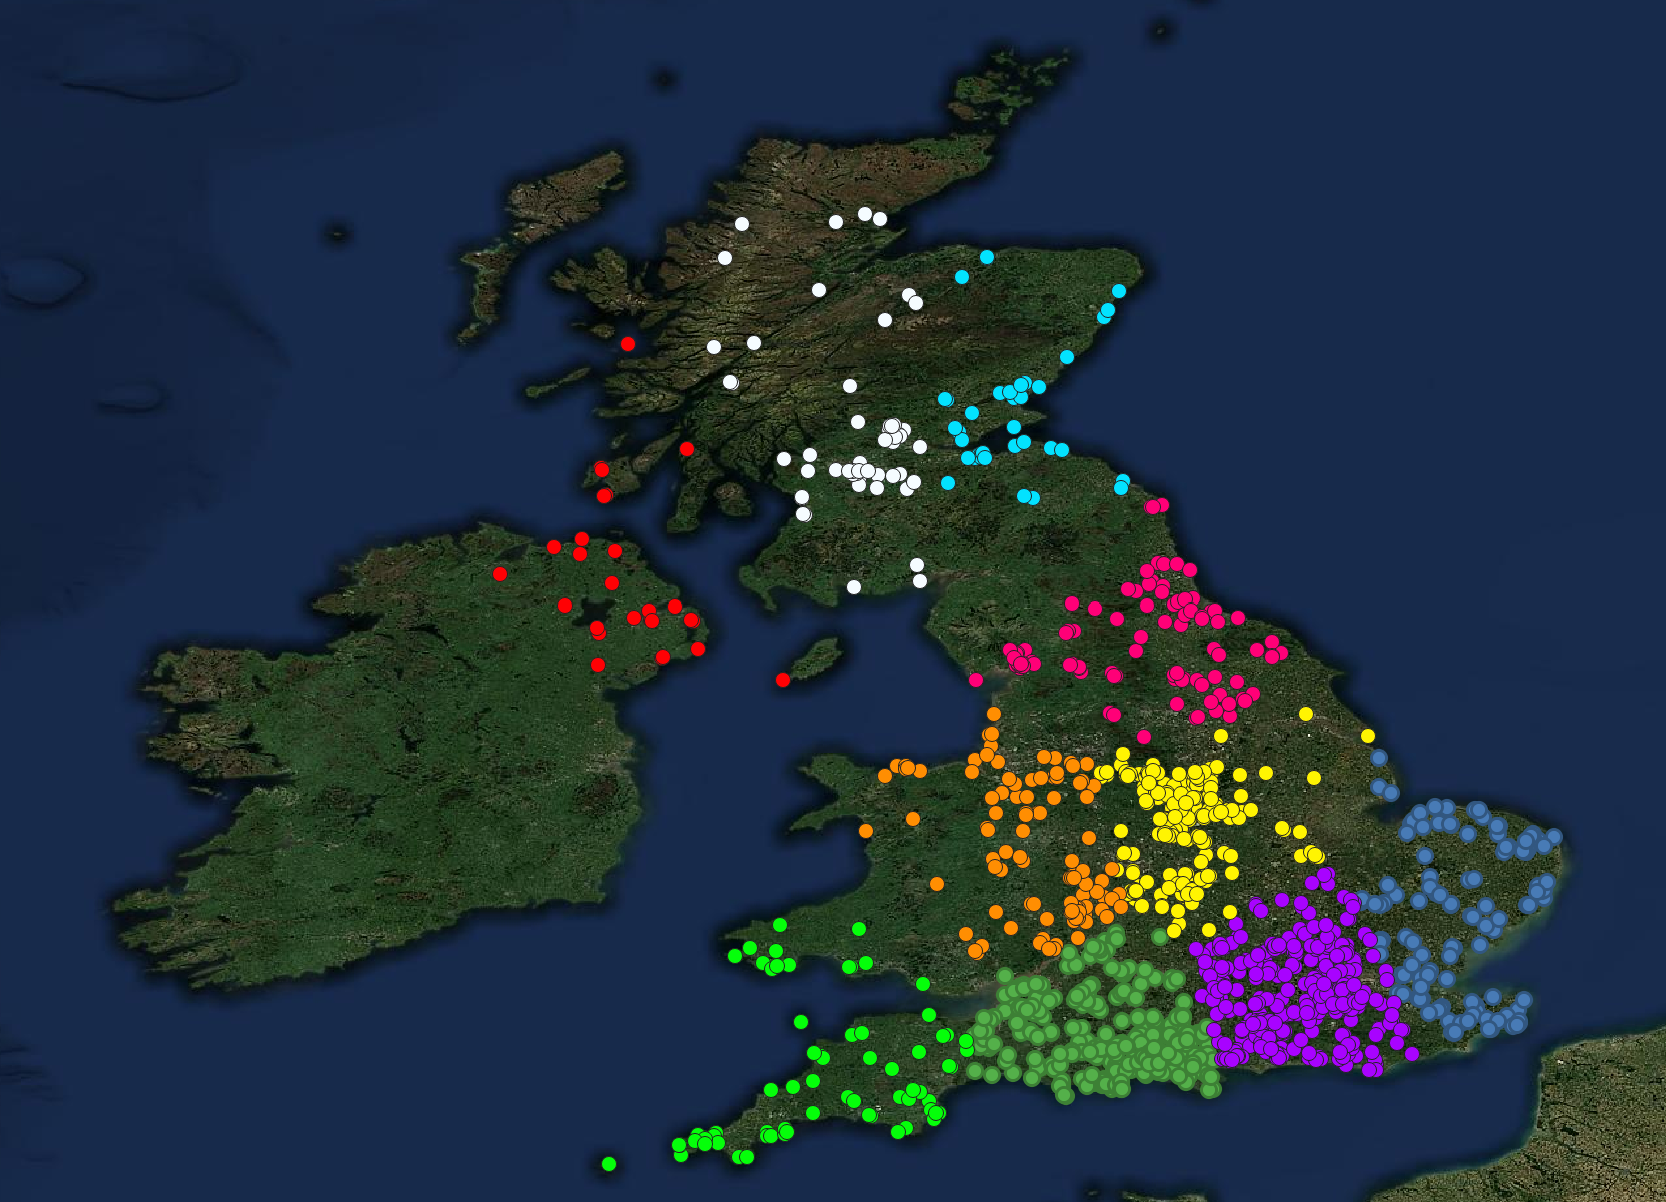
\includegraphics[width=\textwidth]{Images/Spatial_CV_visual.png}
    \caption{2020 UKBMS dataset - Spatial cross-validation folds.}
    \label{fig:spatial-cv-distribution}
\end{subfigure}

\caption{Comparison between the random and spatial cross-validation folds on the 2020 UKBMS dataset.}
\label{fig:comparison-of-ukbms-data-distribution-across-cv-strategies}
\end{figure}


\subsubsection{GLM}\label{subsubsection:glm-cv-comparison}
We first evaluate the GLM model by visualizing the distribution of the GLM's predicted species richness distribution compared to the observed species richness distribution across the test folds for both random and spatial 10-fold cross-validation strategies. This is shown in Figure~\ref{fig:glm-predicted-vs-observed-distribution-across-cv-strategies}, and we can see that they are similar especially if we just look at the mean and standard deviation. The mean and standard deviation for the random cross-validation strategy are \(18.54\) and \(3.49\) respectively, while the mean and standard deviation for the spatial cross-validation strategy are \(18.41\) and \(3.58\) respectively, which the true mean and standard deviation are \(18.54\) and \(6.10\) respectively. However, the distribution of the spatial cross-validation strategy appears to overlap with the true distribution more than the distribution of the random cross-validation strategy. If we look at the plots of the observed vs. predicted species richness across the test folds for both random and spatial cross-validation strategies in Figure~\ref{fig:glm-observed-vs-predicted-across-cv-strategies} we can see a different story. The GLM performs better across the random cross-validation strategy compared to the spatial cross-validation strategy as the points demonstrate a more positive trend and are closer to the 1:1 line. Points in Figure\ref{fig:GLM-spatial-cv-observed-vs-predicted-plots} are not as close to the 1:1 line and for each species richness value there is a wider spread of predicted species richness values compared to the random cross-validation strategy in Figure~\ref{fig:GLM-random-cv-observed-vs-predicted-plots}.


\begin{figure}[H]
\centering

\begin{subfigure}{0.48\textwidth}
    \centering
    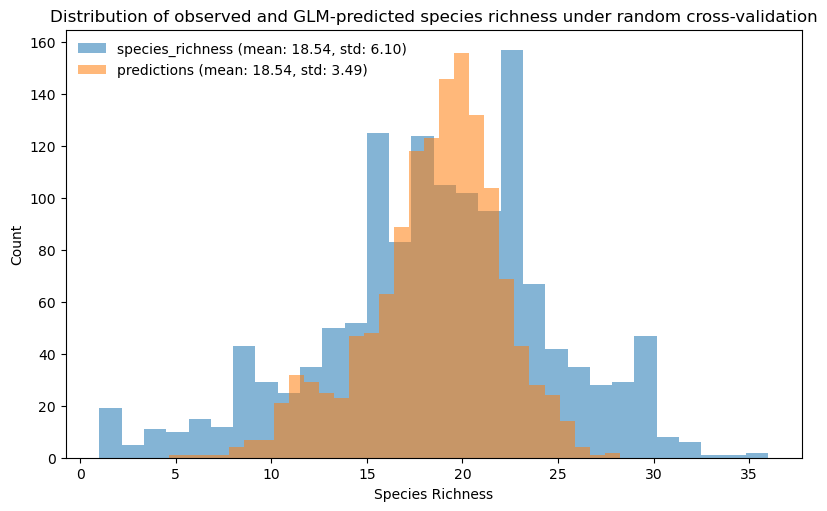
\includegraphics[width=\textwidth]{Images/GLM_spatial/GLM_random_hists.png}
    \caption{Distribution of observed species richness and predicted species richness across the test sets for the random cross-validation strategy.}
    \label{fig:GLM-random-cv-predicted-vs-observed-distribution}
\end{subfigure}
\hfill
\begin{subfigure}{0.48\textwidth}
    \centering
    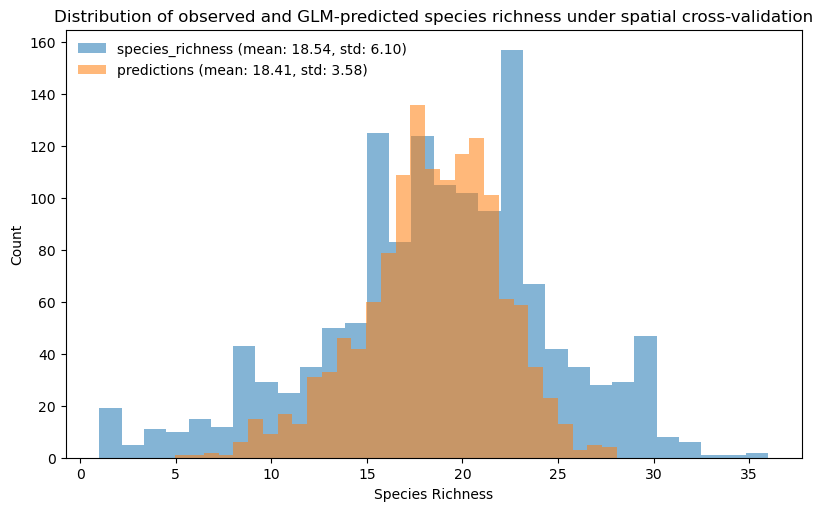
\includegraphics[width=\textwidth]{Images/GLM_spatial/GLM_spatial_hists.png}
    \caption{Distribution of observed species richness and predicted species richness across the test sets for the spatial cross-validation strategy.}
    \label{fig:GLM-spatial-cv-predicted-vs-observed-distribution}
\end{subfigure}

\caption{Comparison between the distribution of observed species richness and predicted species richness between random and spatial cross-validation strategies for the GLM model.}
\label{fig:glm-predicted-vs-observed-distribution-across-cv-strategies}
\end{figure}

\begin{figure}[H]
\centering

\begin{subfigure}{0.48\textwidth}
    \centering
    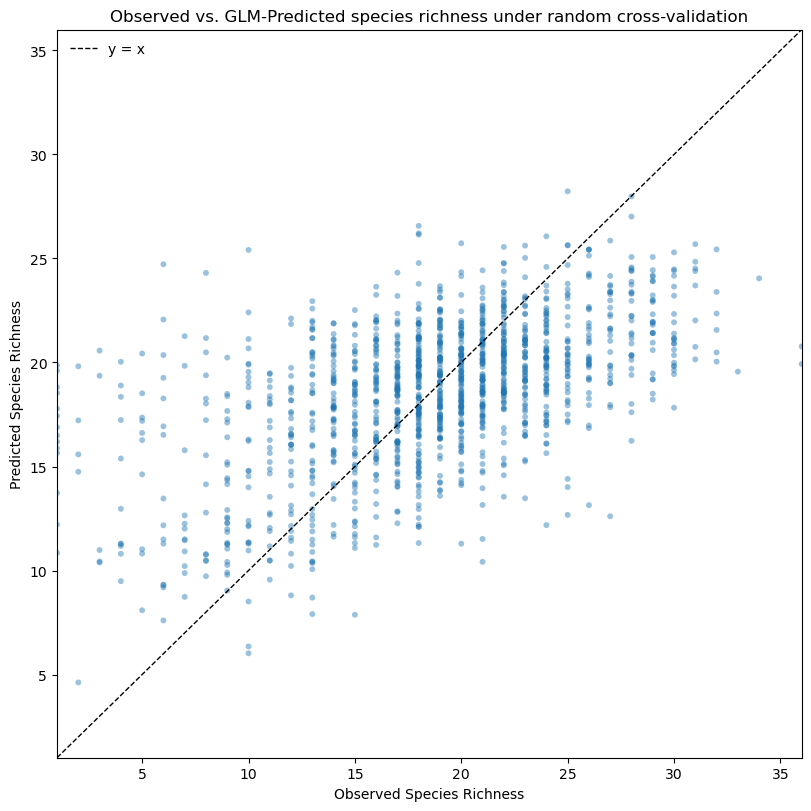
\includegraphics[width=\textwidth]{Images/GLM_spatial/GLM_calibration_plot_random.png}
    \caption{Observed species richness vs. predicted species richness for the random cross-validation strategy \(R^2 = 0.295\).}
    \label{fig:GLM-random-cv-observed-vs-predicted-plots}
\end{subfigure}
\hfill
\begin{subfigure}{0.48\textwidth}
    \centering
    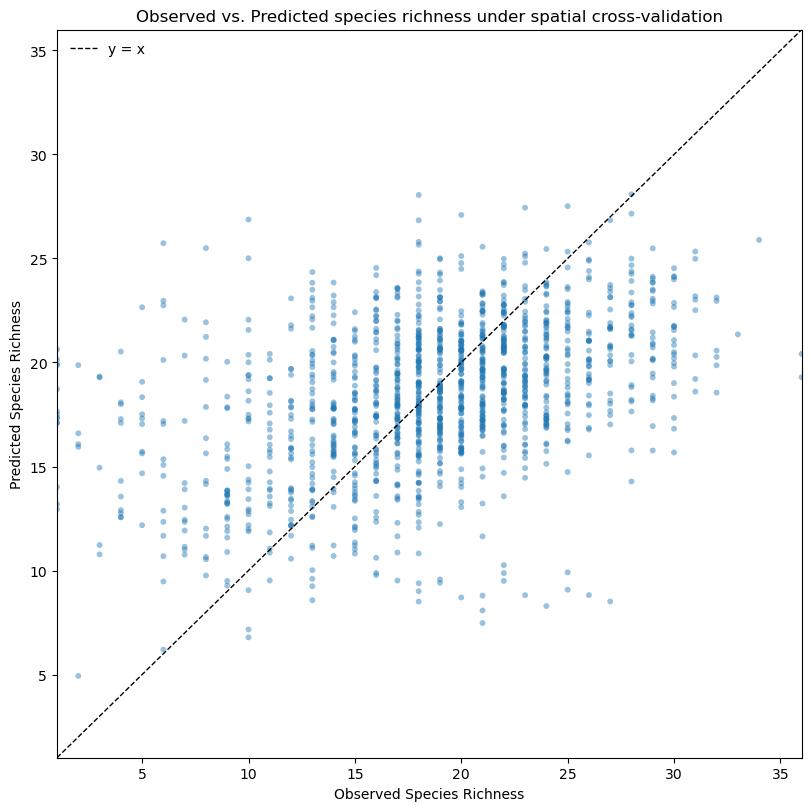
\includegraphics[width=\textwidth]{Images/GLM_spatial/GLM_calibration_plot_spatial.png}
    \caption{Observed species richness vs. predicted species richness for the spatial cross-validation strategy \(R^2 = 0.155\).}
    \label{fig:GLM-spatial-cv-observed-vs-predicted-plots}
\end{subfigure}

\caption{Comparison between observed species richness vs. predicted species richness between random and spatial cross-validation strategies for the GLM model.}
\label{fig:glm-observed-vs-predicted-across-cv-strategies}
\end{figure}

Table~\ref{tab:glm-cv-strategy-comparison} presents the performance comparison across the calculated metrics along with a weighted mean, weighted standard deviation, and pooled metrics. We can see that the GLM performs better with the random cross-validation strategy compared to the spatial cross-validation strategy across all metrics. This is in line with previous studies that have measured cross-validation performance for different models \parencite{cai2023} along with what was expected \parencite{roberts2017}. There are small differences present in the random cross-validation strategy for the weighted and unweighted metrics due to the number of sites not being perfectly divisible by 10, or the number of folds. 

Note worthy results are that the mean \(R^2\) values are negative from the spatial cross-validation strategy except for the pooled mean. This implies that the model performs worse than a horizontal line fitted to the test data sets data. This has to do with the calculation of the \(R^2\) across the different folds as the variance within the test fold can be small and extreme predictions far from the test mean would then result in negative \(R^2\) values. This can happen when the distribution of the test set is different from the training set which is likely the case here due to the spatial cross-validation. If instead we look at the pooled \(R^2\) under spatial cross-validation, which would correspond to the \(R^2\) of the plot in Figure~\ref{fig:GLM-spatial-cv-observed-vs-predicted-plots}, we can see that the \(R^2\) value is weakly positive. 

\begin{table}[ht]
\centering
\small
\caption{Performance comparison for the GLM under random and spatial cross-validation. WM = weighted mean, P = pooled metric calculation, W Std. = weighted standard deviation. Bold values indicate the best value within each metric table.}
\label{tab:glm-cv-strategy-comparison}
\begin{tabular}{llrrrrrrr}
\toprule
\textbf{Metric} & \textbf{CV strategy} & \textbf{Mean} & \textbf{Std.} & \textbf{WM} & \textbf{W Std.} & \textbf{P} & \textbf{Median} & \textbf{IQR} \\
\midrule
\multirow{2}{*}{\(R^2\)}
& GLM Random CV & \textbf{0.291} & \textbf{0.069} & \textbf{0.291} & \textbf{0.065} & \textbf{0.295} & \textbf{0.281} & \textbf{0.118} \\
& GLM Spatial CV & -0.616 & 0.711 & -0.749 & 0.655 & 0.156 & -0.353 & 0.917 \\

\addlinespace
\multirow{2}{*}{RMSE}
& GLM Random CV & \textbf{5.110} & \textbf{0.434} & \textbf{5.110} & \textbf{0.412} & \textbf{5.126} & \textbf{5.184} & \textbf{0.431} \\
& GLM Spatial CV & 5.655 & 0.837 & 6.041 & 0.883 & 5.612 & 5.412 & 1.468 \\

\addlinespace
\multirow{2}{*}{MAPE}
& GLM Random CV & \textbf{0.446} & \textbf{0.161} & \textbf{0.446} & \textbf{0.152} & \textbf{0.446} & \textbf{0.463} & \textbf{0.196} \\
& GLM Spatial CV & 0.653 & 0.411 & 0.779 & 0.451 & 0.480 & 0.511 & 0.485 \\

\addlinespace
\multirow{2}{*}{SMAPE}
& GLM Random CV & \textbf{0.239} & \textbf{0.024} & \textbf{0.239} & \textbf{0.023} & \textbf{0.239} & \textbf{0.240} & \textbf{0.023} \\
& GLM Spatial CV & 0.312 & 0.095 & 0.335 & 0.064 & 0.259 & 0.332 & 0.144 \\

\bottomrule
\end{tabular}
\end{table}

As we can see, there are large variations in the performance of the GLM depending on the cross-validation strategy used. If we look at a visual comparison of the \(R^2\), RMSE, MAPE, and SMAPE values across the random and spatial cross-validation strategies in Figures~\ref{fig:glm-cv-strategy-comparison-metrics} these differences are more pronounced. Notability the spread of the performance metrics under spatial cross validation is significantly higher. Model perform drops across board under the spatial cross-validation strategy compared to the random cross-validation strategy.

\begin{figure}[H]
\centering

\begin{subfigure}{0.48\textwidth}
    \centering
    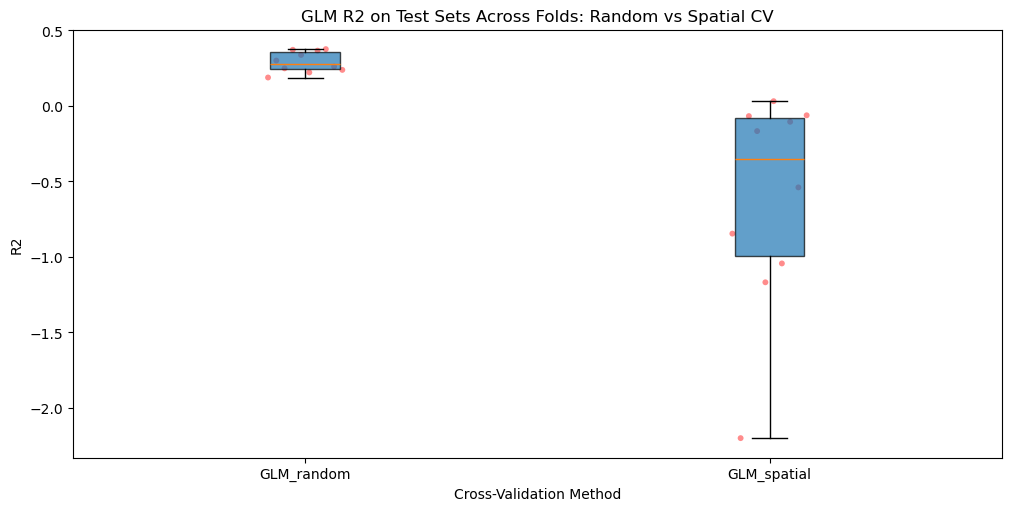
\includegraphics[width=\textwidth]{Images/GLM_spatial/GLM_R2_random_vs_spatial.png}
    \caption{\(R^2\)}
    \label{fig:glm-r2-random-vs-spatial}
\end{subfigure}
\hfill
\begin{subfigure}{0.48\textwidth}
    \centering
    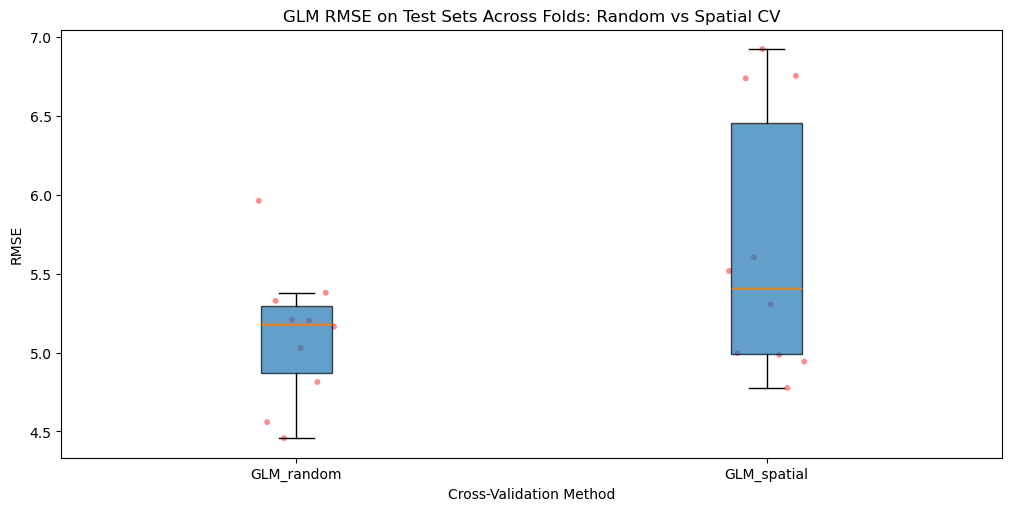
\includegraphics[width=\textwidth]{Images/GLM_spatial/GLM_RMSE_random_vs_spatial.png}
    \caption{RMSE}
    \label{fig:glm-rmse-random-vs-spatial}
\end{subfigure}

\vspace{0.5cm}

\begin{subfigure}{0.48\textwidth}
    \centering
    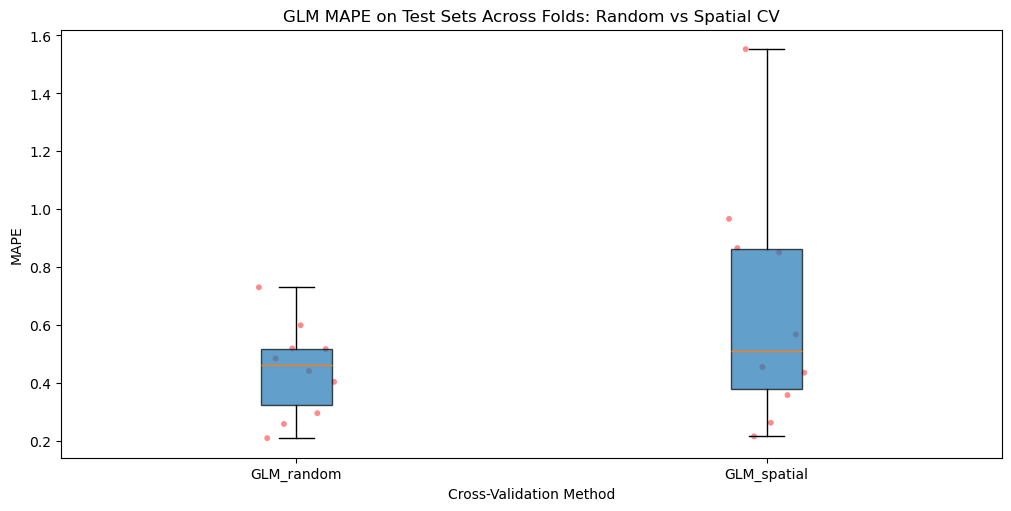
\includegraphics[width=\textwidth]{Images/GLM_spatial/GLM_mape_random_vs_spatial.png}
    \caption{MAPE}
    \label{fig:glm-mape-random-vs-spatial}
\end{subfigure}
\hfill
\begin{subfigure}{0.48\textwidth}
    \centering
    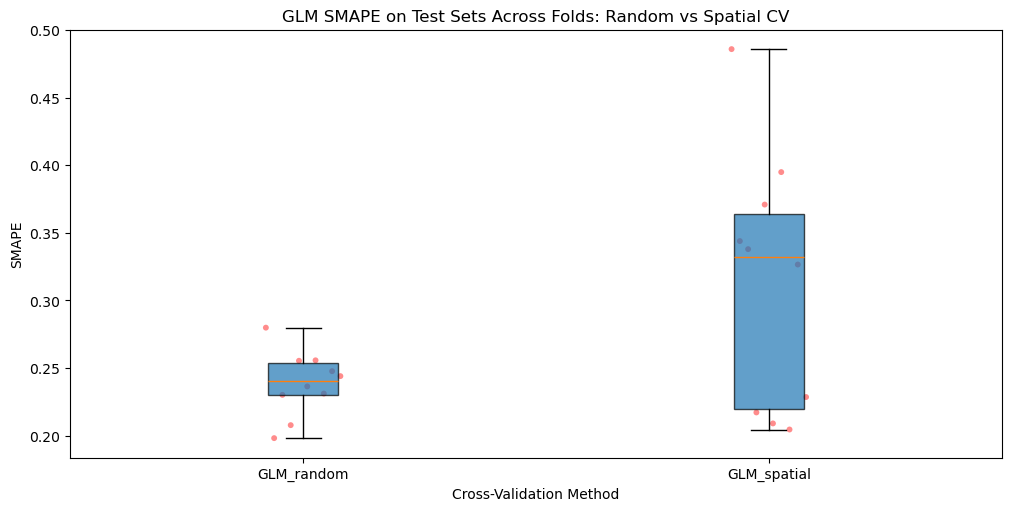
\includegraphics[width=\textwidth]{Images/GLM_spatial/GLM_smape_random_vs_spatial.png}
    \caption{SMAPE}
    \label{fig:glm-smape-random-vs-spatial}
\end{subfigure}

\caption{Comparison of GLM performance metrics across random and spatial cross-validation strategies.}
\label{fig:glm-cv-strategy-comparison-metrics}
\end{figure}

\subsubsection{CatBoost}\label{subsubsection:catboost-cv-comparison}
Second, we evaluate a comparison of random vs. spatial cross-validation strategies applied to the CatBoost model. We look at a distribution of CatBoost's predicted species richness distribution compared to the observed species richness distribution across the test sets for both random and spatial cross-validation strategies. This is shown in Figure~\ref{fig:catboost-predicted-vs-observed-distribution-across-cv-strategies} and we can see that the random cross-validation trained model is closer in mean to the true distribution and is more spread out compared to the spatial cross-validation trained model. The mean and standard deviation for the random cross-validation strategy are \(18.56\) and \(4.04\) respectively, while the mean and standard deviation for the spatial cross-validation strategy are \(17.99\) and \(3.22\) respectively, which the true mean and standard deviation are \(18.54\) and \(6.10\) respectively.

\begin{figure}[H]
\centering

\begin{subfigure}{0.48\textwidth}
    \centering
    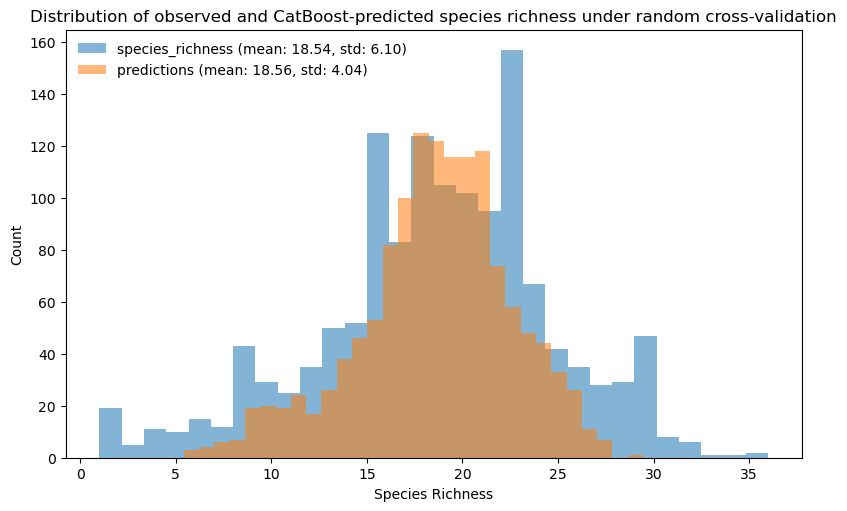
\includegraphics[width=\textwidth]{Images/CatBoost/CatBoost_random_hists.png}
    \caption{Distribution of observed species richness and predicted species richness across the test sets for the random cross-validation strategy.}
    \label{fig:CatBoost-random-cv-predicted-vs-observed-distribution}
\end{subfigure}
\hfill
\begin{subfigure}{0.48\textwidth}
    \centering
    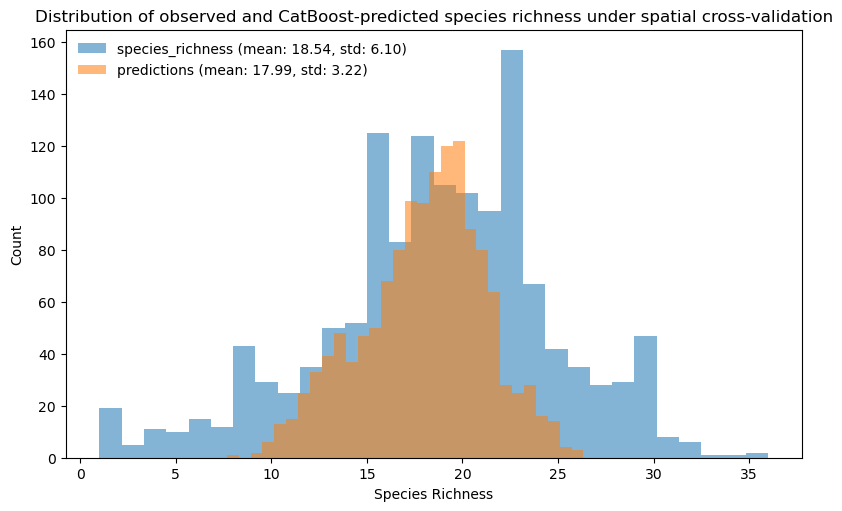
\includegraphics[width=\textwidth]{Images/CatBoost/CatBoost_spatial_hists.png}
    \caption{Distribution of observed species richness and predicted species richness across the test sets for the spatial cross-validation strategy.}
    \label{fig:CatBoost-spatial-cv-predicted-vs-observed-distribution}
\end{subfigure}

\caption{Comparison between the distribution of observed species richness and predicted species richness between 10-fold random and spatial cross-validation strategies for the CatBoost model.}
\label{fig:catboost-predicted-vs-observed-distribution-across-cv-strategies}
\end{figure}

If we also look at the plots of the observed vs. predicted species richness across the test sets for both random and spatial cross-validation strategies in Figure~\ref{fig:catboost-observed-vs-predicted-across-cv-strategies} we can further see a difference in performance across the two strategies. The random cross-validation strategy demonstrates a more defined positive trend; whereas, the spatial cross-validation strategy does not demonstrates as strong of a trend and the data points are more spread out across the range of observed species richness values.

\begin{figure}[H]
\centering

\begin{subfigure}{0.48\textwidth}
    \centering
    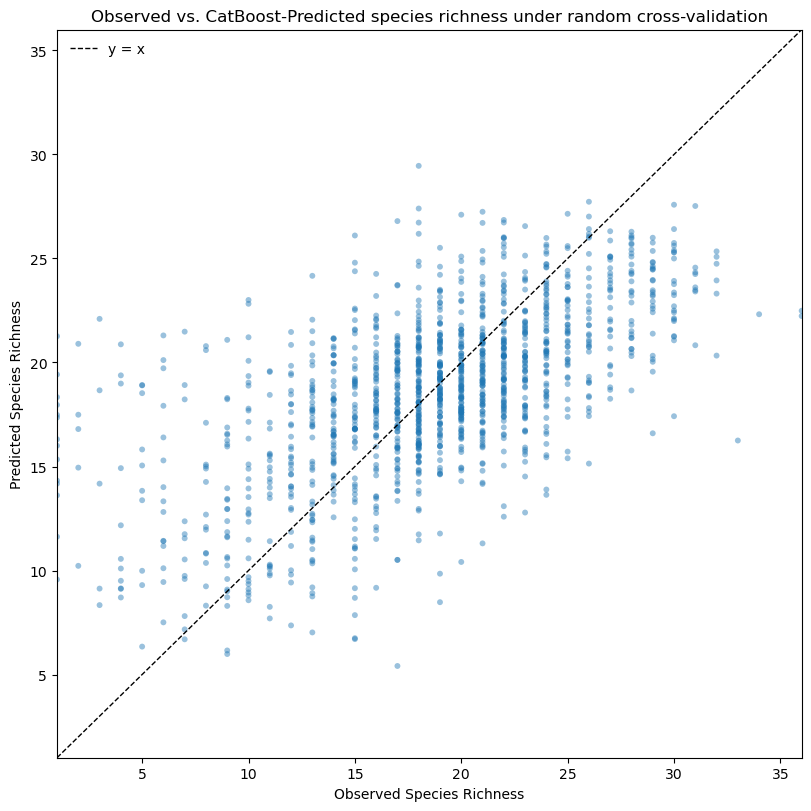
\includegraphics[width=\textwidth]{Images/CatBoost/CatBoost_calibration_plot_random.png}
    \caption{Observed species richness vs. predicted species richness for the random cross-validation strategy \(R^2 = 0.376\).}
    \label{fig:CatBoost-random-cv-observed-vs-predicted-plots}
\end{subfigure}
\hfill
\begin{subfigure}{0.48\textwidth}
    \centering
    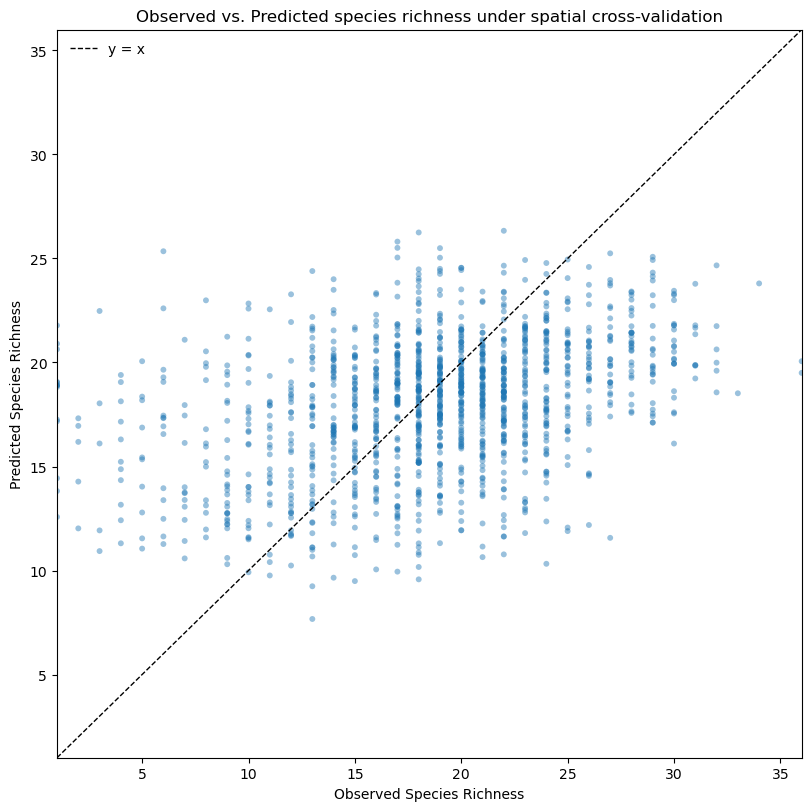
\includegraphics[width=\textwidth]{Images/CatBoost/CatBoost_calibration_plot_spatial.png}
    \caption{Observed species richness vs. predicted species richness for the spatial cross-validation strategy \(R^2 = 0.109\).}
    \label{fig:CatBoost-spatial-cv-observed-vs-predicted-plots}
\end{subfigure}

\caption{Comparison between observed species richness vs. predicted species richness between random and spatial cross-validation strategies for the CatBoost model.}
\label{fig:catboost-observed-vs-predicted-across-cv-strategies}
\end{figure}

Table~\ref{tab:catboost-cv-strategy-comparison} displays the performance comparison across the metrics along with weighted mean, weighted standard deviation, and pooled metrics. We can see that the CatBoost model performs better across the random cross-validation strategy compared to the spatial cross-validation strategy for all metrics again in line with what we expect \parencite{roberts2017}. However, we see a very large drop in \(R^2\) values when moving from random to spatial cross-validation strategies. The plots in Figure~\ref{fig:catboost-observed-vs-predicted-across-cv-strategies} confirm this as there is a very noticeable drop in the strength of the positive trend between observed and predicted species richness values when moving from random to spatial cross-validation strategies. We also observe negative \(R^2\) values in the spatial cross-validation strategy which can occur under low test set variance and extreme predictions far from the test mean, which is likely the case here due to the spatial cross-validation strategy.

\begin{table}[ht]
\centering
\small
\caption{Performance comparison for the CatBoost under random and spatial cross-validation. WM = weighted mean, P = pooled metric calculation, W Std. = weighted standard deviation. Bold values indicate the best value within each metric table.}
\label{tab:catboost-cv-strategy-comparison}
\begin{tabular}{llrrrrrrr}
\toprule
\textbf{Metric} & \textbf{CV strategy} & \textbf{Mean} & \textbf{Std.} & \textbf{WM} & \textbf{W Std.} & \textbf{P} & \textbf{Median} & \textbf{IQR} \\
\midrule
\multirow{2}{*}{\(R^2\)}
& CatBoost Random CV & \textbf{0.374} & \textbf{0.083} & \textbf{0.374} & \textbf{0.078} & \textbf{0.376} & \textbf{0.397} & \textbf{0.122} \\
& CatBoost Spatial CV & -0.958 & 1.552 & -1.019 & 1.391 & 0.109 & -0.343 & 0.666 \\

\addlinespace
\multirow{2}{*}{RMSE}
& CatBoost Random CV & \textbf{4.800} & \textbf{0.482} & \textbf{4.800} & \textbf{0.458} & \textbf{4.821} & \textbf{4.813} & \textbf{0.343} \\
& CatBoost Spatial CV & 5.912 & 0.685 & 6.193 & 0.609 & 5.761 & 5.697 & 0.725 \\

\addlinespace
\multirow{2}{*}{MAPE}
& CatBoost Random CV & \textbf{0.425} & \textbf{0.160} & \textbf{0.425} & \textbf{0.152} & \textbf{0.424} & \textbf{0.430} & \textbf{0.177} \\
& CatBoost Spatial CV & 0.694 & 0.458 & 0.822 & 0.493 & 0.498 & 0.467 & 0.627 \\

\addlinespace
\multirow{2}{*}{SMAPE}
& CatBoost Random CV & \textbf{0.227} & \textbf{0.024} & \textbf{0.227} & \textbf{0.023} & \textbf{0.227} & \textbf{0.226} & \textbf{0.021} \\
& CatBoost Spatial CV & 0.333 & 0.103 & 0.347 & 0.075 & 0.273 & 0.337 & 0.175 \\
\bottomrule
\end{tabular}
\end{table}

If we look at a comparison of the \(R^2\), RMSE, MAPE, and SMAPE box-plots across the random and spatial cross-validation strategies in Figure~\ref{fig:catboost-cv-strategy-comparison-rmse} we can see a clear difference in the median and interquartile range of the models. Notability the spread of the data under spatial cross validation is significantly higher. Model performance drops across the spatial cross-validation strategy compared to the random cross-validation strategy across all metrics. This is again most prominent in the \(R^2\) values in Figure\ref{fig:catboost-r2-random-vs-spatial}, where the random cross validation box-plot barely fits on the screen with the spatial cross-validation box-plot having a much wider range of \(R^2\) values that extend far into negative values.

\begin{figure}[H]
\centering

\begin{subfigure}{0.48\textwidth}
    \centering
    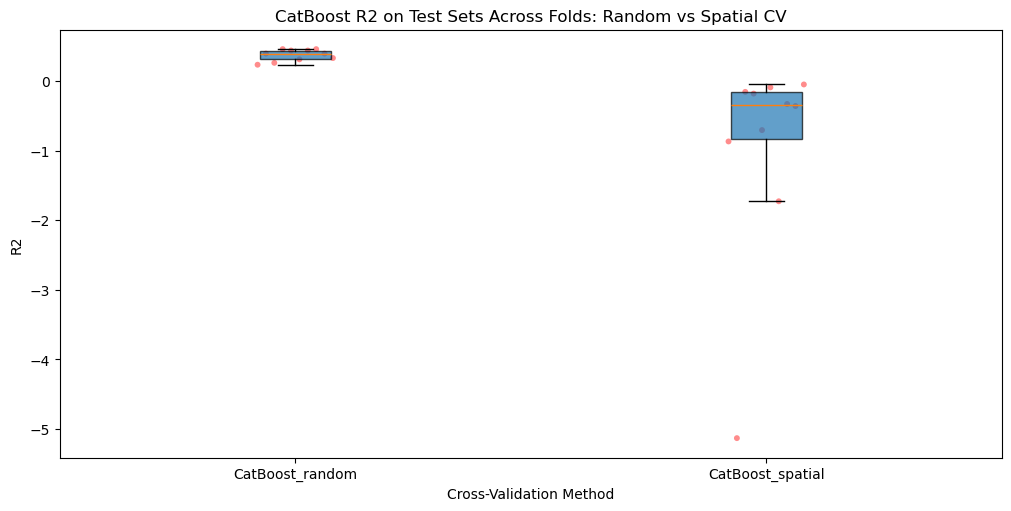
\includegraphics[width=\textwidth]{Images/CatBoost/CatBoost_r2_random_vs_spatial.png}
    \caption{\(R^2\)}
    \label{fig:catboost-r2-random-vs-spatial}
\end{subfigure}
\hfill
\begin{subfigure}{0.48\textwidth}
    \centering
    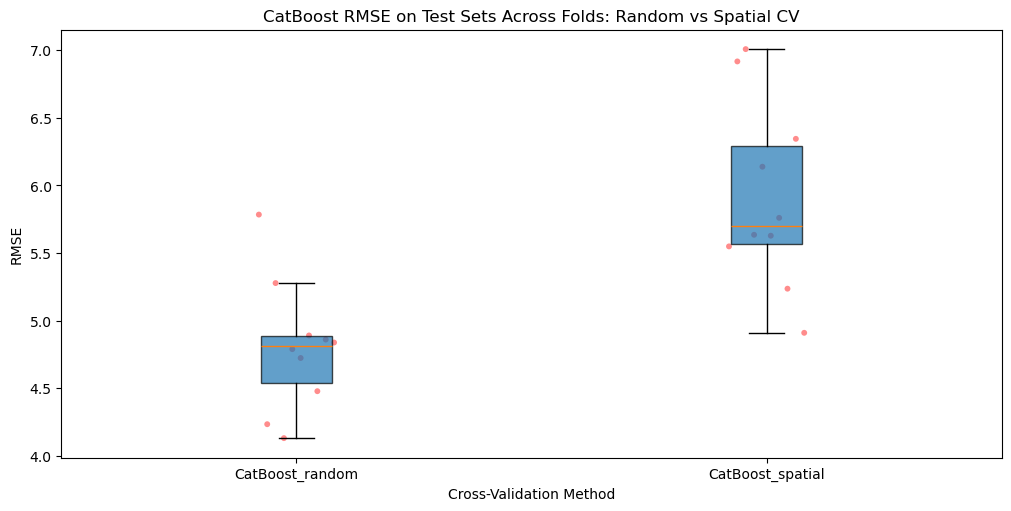
\includegraphics[width=\textwidth]{Images/CatBoost/CatBoost_RMSE_random_vs_spatial.png}
    \caption{RMSE}
    \label{fig:catboost-rmse-random-vs-spatial}
\end{subfigure}

\vspace{0.5cm}

\begin{subfigure}{0.48\textwidth}
    \centering
    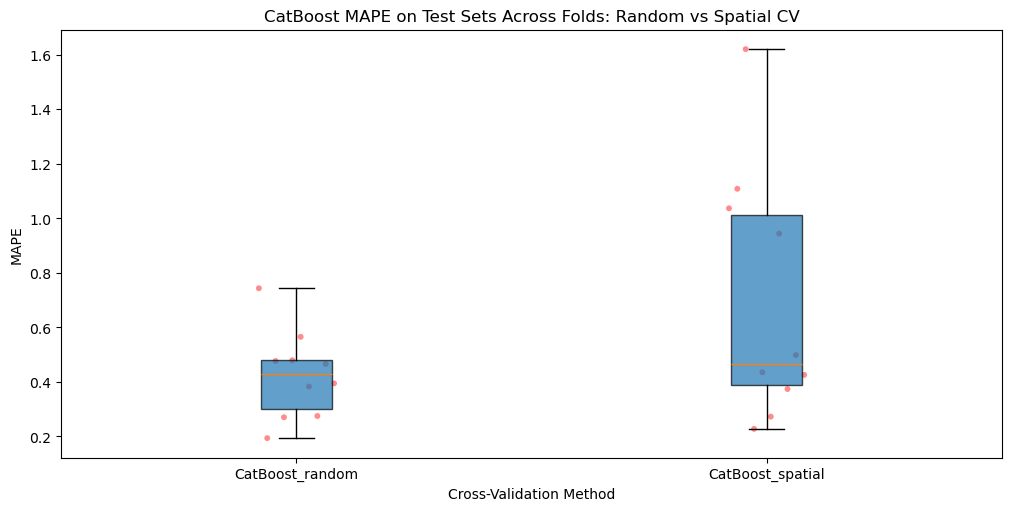
\includegraphics[width=\textwidth]{Images/CatBoost/CatBoost_mape_random_vs_spatial.png}
    \caption{MAPE}
    \label{fig:catboost-mape-random-vs-spatial}
\end{subfigure}
\hfill
\begin{subfigure}{0.48\textwidth}
    \centering
    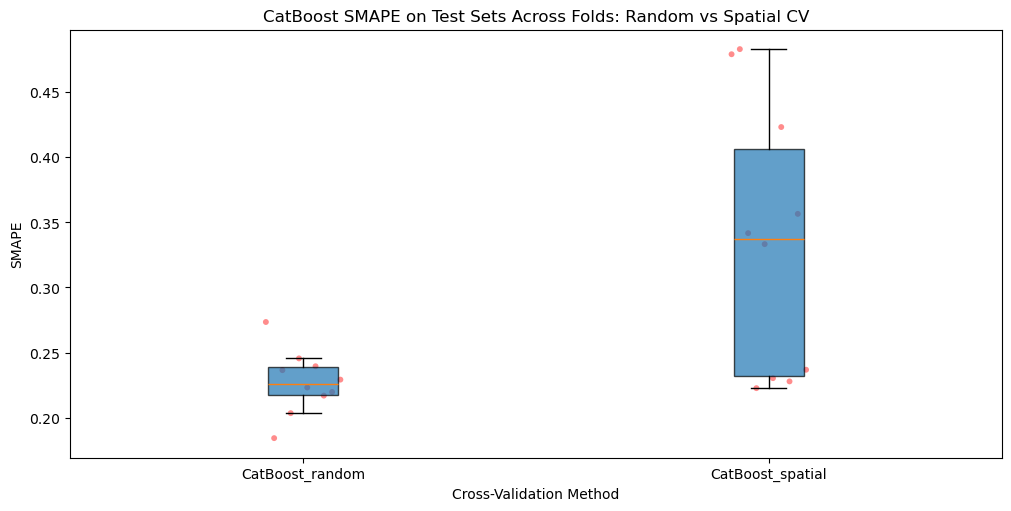
\includegraphics[width=\textwidth]{Images/CatBoost/CatBoost_smape_random_vs_spatial.png}
    \caption{SMAPE}
    \label{fig:catboost-smape-random-vs-spatial}
\end{subfigure}

\caption{Comparison of CatBoost performance metrics across random and spatial cross-validation strategies.}
\label{fig:catboost-cv-strategy-comparison-metrics}
\label{fig:catboost-cv-strategy-comparison-rmse}
\end{figure}

\newpage
\subsection{Limited data scenarios}\label{sec:research-question-3}
